In Versuch DT3 wurden verschiedene Flip-Flop-Arten (SR-Flip-Flop, E-Flip-Flop, D-Flip-Flop) untersucht. Dabei sollten Unterschiede zwischen den Flip-Flops festgestellt werden. \par
In der Vorbereitung wurden dazu zunächst Wahrheitstabellen und KV-Diagramme der Flip-Flops ausgefüllt um die konjunktive und disjunktive Normalform zu bilden. Um die disjunktive Normalform zu erhalten, wurden die Einsen im KV-Diagramm zusammenfasst. Um auf die konjunktive Normalform zu kommen, wurde die disjunktive Normalform negiert. Eine Alternative um die konjunktive Normalform zu bilden ist, die Nullen im KV-Diagramm zusammenzufassen. Mit Hilfe der beiden Normalformen wurden Schaltungen in NOR- und NAND-Technik entwickelt. \par
Bei der Versuchsdurchführung wurden mit Hilfe eines HPS-Boards, wie in Abbildung 2.1 zu sehen, ICs und Laborleitungen die verschiedenen Schaltungen aufgebaut und auf ihre Funktion getestet. Dabei musste die Pin Belegung der ICs beachtet werden. \par
Alle in der Versuchsanleitung beschriebenen Aufgaben konnten ohne größere Probleme in der gegebenen Zeit durchgeführt werden.\\
\vspace{10mm}
\begin{center}
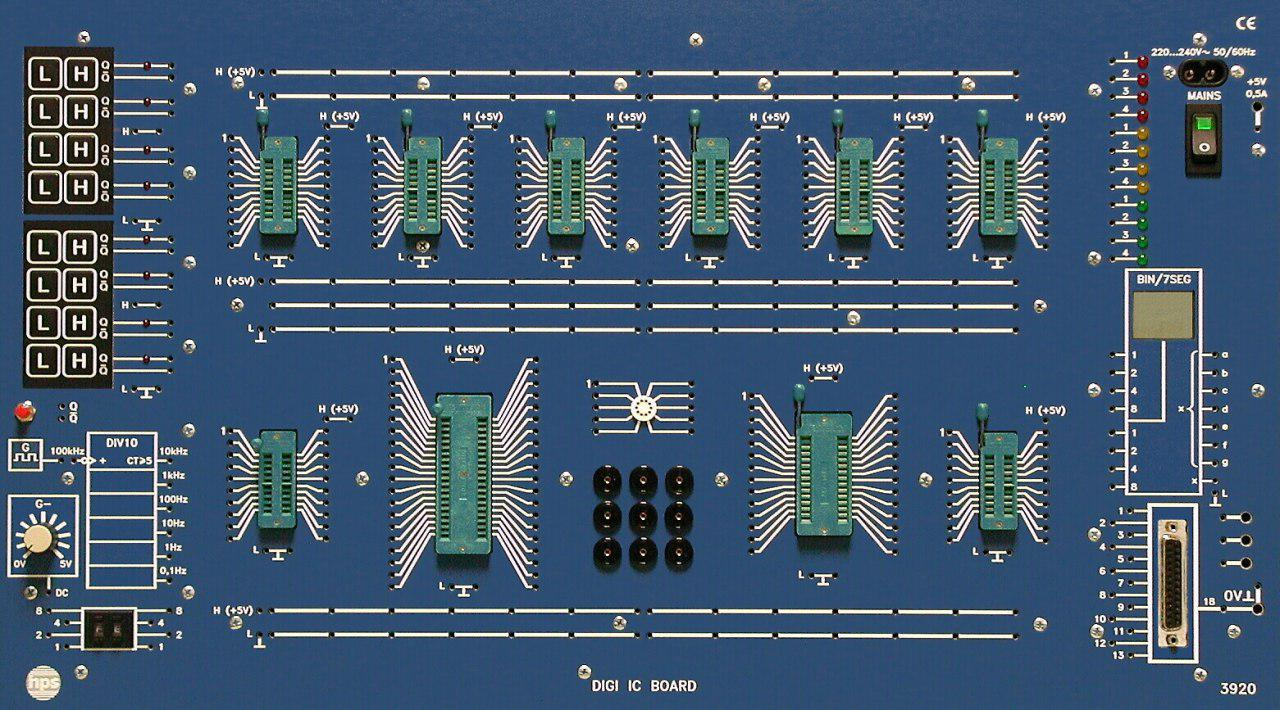
\includegraphics[width=0.75\columnwidth]{DT3Graphics/HPSBoard.jpg}
\captionof{figure}{HPS-Board}
\end{center}
